\documentclass[a4paper, twoside,openright]{report}

\usepackage[a4paper,top=3cm,bottom=3cm,left=3cm,right=3cm]{geometry}
\usepackage[fontsize=13pt]{scrextend}
\usepackage[english,italian]{babel}
\usepackage[fixlanguage]{babelbib}
\usepackage[utf8]{inputenc}
\usepackage[T1]{fontenc}
\usepackage{lipsum}
\usepackage{rotating}
\usepackage{fancyhdr}
\usepackage{amssymb}
\usepackage{amsmath}
\usepackage{amsthm}
\usepackage{lmodern}
\usepackage{graphicx}
\usepackage[dvipsnames]{xcolor}
\usepackage{listings}
\usepackage{listings}
\usepackage{xparse}
\usepackage{hyperref}
\usepackage[normalem]{ulem}
\usepackage{float}


\definecolor{dkgreen}{rgb}{0,0.6,0}
\definecolor{gray}{rgb}{0.5,0.5,0.5}
\definecolor{mauve}{rgb}{0.58,0,0.82}

\lstset{frame=tb,
  language=Java,
  aboveskip=3mm,
  belowskip=3mm,
  showstringspaces=false,
  columns=flexible,
  basicstyle={\small\ttfamily},
  numbers=none,
  numberstyle=\tiny\color{gray},
  keywordstyle=\color{blue},
  commentstyle=\color{dkgreen},
  stringstyle=\color{mauve},
  breaklines=true,
  breakatwhitespace=true,
  tabsize=3
}

\lstdefinelanguage{JavaScript}{
  keywords={typeof, new, true, false, catch, function, return, null, catch, switch, var, if, in, while, do, else, case, break},
  keywordstyle=\color{blue}\bfseries,
  ndkeywords={class, export, boolean, throw, implements, import, this},
  ndkeywordstyle=\color{darkgray}\bfseries,
  identifierstyle=\color{black},
  sensitive=false,
  comment=[l]{//},
  morecomment=[s]{/*}{*/},
  commentstyle=\color{purple}\ttfamily,
  stringstyle=\color{red}\ttfamily,
  morestring=[b]',
  morestring=[b]"
}

\lstset{
   language=JavaScript,
   extendedchars=true,
   basicstyle=\footnotesize\ttfamily,
   showstringspaces=false,
   showspaces=false,
   numbers=left,
   numberstyle=\footnotesize,
   numbersep=9pt,
   tabsize=2,
   breaklines=true,
   showtabs=false,
   captionpos=b
}

\NewDocumentCommand{\codeword}{v}{%
\texttt{\textcolor{blue}{#1}}%
}

% -----------------------------------------------------------------

\pagestyle{fancy}
\fancyhf{}
\lhead{\rightmark}
\rhead{\textbf{\thepage}}
\fancyfoot{}
\setlength{\headheight}{12.5pt}

% Rimuove il numero di pagina all'inizio dei capitoli
\fancypagestyle{plain}{
  \fancyfoot{}
  \fancyhead{}
  \renewcommand{\headrulewidth}{0pt}
}



% Modifica dello stile dei riferimenti, con il testo in cyano
\hypersetup{
    colorlinks,
    linkcolor=CornflowerBlue,
    citecolor=CornflowerBlue
}

\newtheorem{definition}{Definizione}[section]
\newtheorem{theorem}{Teorema}[section]
\providecommand*\definitionautorefname{Definizione}
\providecommand*\theoremautorefname{Teorema}
\providecommand*{\listingautorefname}{Listing}
\providecommand*\lstnumberautorefname{Linea}

\raggedbottom




% -----------------------------------------------------------------
\begin{document}

\begin{titlepage}
\begin{figure}[!htb]
    \centering
    
\includegraphics[keepaspectratio=true,scale=0.5]{images/cherubino.eps}
\end{figure}

\begin{center}
    \LARGE{UNIVERSITÀ DI PISA}
    \vspace{5mm}
    \\ \large{DIPARTIMENTO DI INGEGNERIA DELL'INFORMAZIONE}
    \vspace{5mm}
    \\ \LARGE{Laurea Triennale in Ingegneria Informatica}
\end{center}

\vspace{15mm}
\begin{center}
    {\LARGE{\bf Progetto e realizzazione di una estensione VSCode per il debugging di un nucleo multiprogrammato}
    
\end{center}

\vspace{30mm}

\begin{minipage}[t]{0.47\textwidth}
	{\large{Relatore:}{\normalsize\vspace{3mm}
	\bf\\ \large{Prof: Giuseppe Lettieri} \normalsize\vspace{3mm}\bf \\ \large{Prof: Luigi Leonardi}}}
\end{minipage}
\hfill
\begin{minipage}[t]{0.47\textwidth}\raggedleft
	{\large{Candidato:}{\normalsize\vspace{3mm} \bf\\ \large{Francesco Mignone}}}
\end{minipage}

\vspace{30mm}
\hrulefill
\\\centering{\large{ANNO ACCADEMICO 2023/2024}}

\end{titlepage}


\begin{center}
    \LARGE{\bf Abstract}
    \vspace{5mm}
\end{center}

Questo elaborato descrive la progettazione e l'implementazione di un'estensione per VS Code che facilita il debugging
del nucleo multiprogrammato didattico. Gli obiettivi principali dell'estensione includono la possibilità di
impostare e gestire breakpoints,
visualizzare variabili in tempo reale e eseguire codice passo-passo. Per raggiungere questi
obiettivi, l'estensione utilizza il Debug Adapter Protocol (DAP) per interfacciarsi con strumenti di debugging
tradizionali come GDB.

Il lavoro presentato in questa tesi comprende un'analisi dettagliata dei requisiti funzionali e non funzionali,
l'analisi dell'architettura dell'estensione e l'implementazione delle principali funzionalità.
lo scopo dell'estensione è semplificare significativamente il processo di debugging del nucleo,
offrendo un'interfaccia utente intuitiva e funzionalità avanzate di debugging.

Vengono inoltre discusse le limitazioni dell'estensione e vengono proposte possibili direzioni per futuri miglioramenti,
tra cui l'aggiunta di ulteriori funzionalità e l'ottimizzazione delle prestazioni.

\tableofcontents
\setcounter{page}{1}
\chapter{Introduzione}
TODO: Forse emglio togliere la subsection
\section{Contesto e motivazione}
Il nucleo di un sistema operativo è il componente software fondamentale che gestisce le risorse hardware e software. A causa della sua complessità e della sua importanza critica, il debugging del nucleo è un compito altamente specialistico che richiede strumenti potenti e una profonda comprensione del sistema. Tuttavia, gli strumenti tradizionali come GDB e QEMU possono essere difficili da utilizzare, soprattutto per i nuovi sviluppatori o per coloro che preferiscono interfacce grafiche più intuitive.

Visual Studio Code (VSCode) è un editor di codice sorgente open-source sviluppato da Microsoft. VS Code è diventato molto popolare tra gli sviluppatori grazie alla sua facilità d'uso e alla sua capacità di supportare molti linguaggi di programmazione grazie alla sua vasta gamma di estensioni disponibili. Tuttavia, al momento della scrittura di questa tesi, non esiste un'estensione dedicata per il debugging del nucleo didattico su VSCode.

L'obiettivo di questa tesi è sviluppare un'estensione per VS Code che renda il debugging del nucleo più accessibile e intuitivo, permettendo agli sviluppatori di beneficiare dell'ambiente user-friendly di VSCode senza rinunciare alla potenza degli strumenti tradizionali.

\chapter{Ambiente e strumenti}
\section{Il debugger - GDB e QEMU}
\subsection{Quick emulator - QEMU}
QEMU é un emulatore open-source, permette di emulare l'architettura di un processore. Permette quindi l'utilizzo di vari sistemi operativi ad un livello di virtualizzazzione Kernel-Based (Kernel Vitual Machine - KVM) con il beneficio di prestazioni vicine all'hardware. Per il nostro utilizzo QEMU emula un sistema x86-64. 
\subsection{GNU Debugger - GDB}
GNU Debugger (GDB) è un debugger portatile, permette quindi di testare e effettuare il debug di programmi. Eseguire il programma in questo ambiente controllato permette al programmatore di tenere traccia dell'esecuzione e monitorare le risorse al fine di individuare un eventuale malfunzionamento nel codice. Per la realizzaione dell'estensione utilizzeremo la funzione di debug remoto per connetterci ad un socket di sistema utilizzato da QEMU per il debug. GDB utilizza delle chiamate di sistema chiamate \codeword{process trace} (\codeword{ptrace}). 

\subsubsection{Breakpoints}
Un breakpoint permette al programma in esecuzione all'interno di un debugger di interrompere il flusso in un determinato punto. Si realizzano sostituendo all'istruzione, alla quale si vuole fermare l'esecuzione, una speciale istruzione la quale solitamente invia un segnale SIGTRAP, il quale verrà catturato dal debugger. Il procedimento di sostituzione è eseguito dal debugger stesso prima di avviare l'esecuzione, nel caso di GDB il programmatore deve eseguire il comando \codeword{break [arg]} dove l'argomento può essere la specifica linea di codice o un simbolo. 

\subsubsection{Continue e Stop}
Tramite i comandi \codeword{continue} e \codeword{stop} possiamo rispettivamente, a seguito di un interruzione, continuare la normale esecuzione del codice oppure interrompere l'esecuzione del programma.

\subsubsection{Step Over}
Permette di proseguire alla prossima istruzione senza entrare nei componenti interni delll'istruzione a cui siamo fermi attualmente.

\subsubsection{Step Into}
Rende possibile seguire il codice riga-per-riga entrando anche nei componenti interni e subroutine.

\subsubsection{Step Out}
Quando all'interno di una subroutine e si vuole risalire al chiamante, il comando \codeword{stepOut} permette di far continuare l'esecuzione fino a ritornare all'istruzione successiva del chiamante.

\subsubsection{Analisi delle variabili}
Durante l'esecuzione vi può essere la necessità di osservare come il valore o il tipo di una variabile cambi. Inoltre é possibile cambiare il valore delle variabili ad esecuzione avviata.

\subsubsection{Call Stack}
Il call stack, o program stack, é una struttura che permette di raccogliere informazioni su tutte le subroutine di un programma in esecuzione. Tale struttura é utile per tenere traccia di quale routine ha il controllo del flusso di istruzioni e a chi deve restituire tale controllo al termine della propria esecuzione.

\subsubsection{Comandi personalizzati}
Ulteriore funzione di GDB è la possibilità di estendere le funzionalità, tramite script in python, come la creazione di comandi personalizzati.

\section{L'architettura del debugger di VS Code}
Tipicamente se si vuole creare un debugger e la sua interfaccia grafica bisogna implementare l'intera applicazione. Microsoft ha realizzato un protocollo che permette di comunicare con i debugger: il Debug Adapter Protocol (DAP). VSCode, o altri applicativi, tramite il DAP si interfaccia non direttamente al debugger ma a un attore intermedio, il Debug Adapter (DA) il quale si occupa di trasformare le richieste dell'applicazione in comandi per il debugger di destinazione.

\begin{figure}[H]
    \centering
    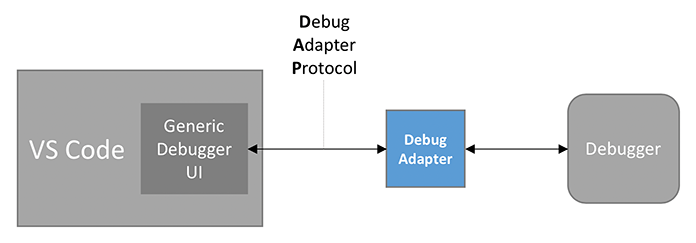
\includegraphics[width=0.7\columnwidth]{images/debug-arch1.png}
    \caption{DAP e DP}
    \label{fig:dap e dp}
\end{figure}

Rende possibile quindi la realizzazione di una generica interfaccia di debug la quale poi si occupa di comunicare con uno o piú DP. Inoltre i Debug Adapters possono essere riutilizzati in diversi ambienti di sviluppo, eliminando la necessitá di crearne uno specifico per ogni esigenza. 

\begin{figure}[H]
    \centering
    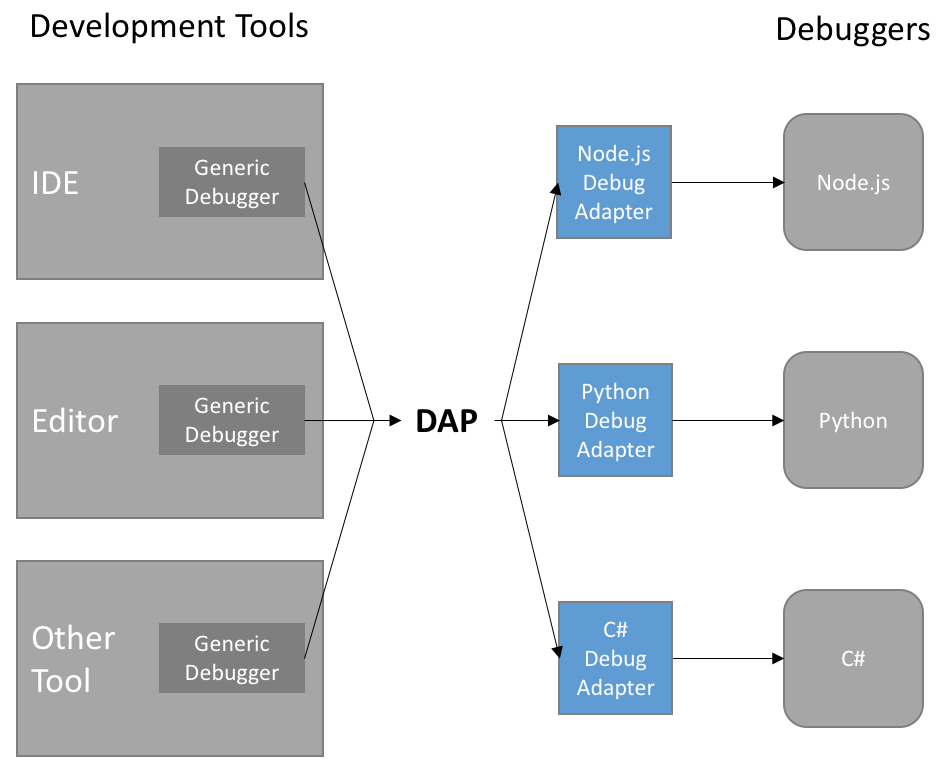
\includegraphics[width=0.7\columnwidth]{images/with-DAP.png}
    \caption{Ambienti di sviluppo multipli}
    \label{fig:Ambienti di sviluppo multipli}
\end{figure}

\subsection{Debug Adapter Protocol e Debug Adapter}

Analizziamo come avviene la connessione e scambio di messaggi tra l'applicativo e il debugger. Gli strumenti di sviluppo possono interagire con il Debug Adapter in due modi:
\begin{itemize}
    \item {
        Modalità a singola sessione: l'applicazione avvia una sessione di debug singola e comunica attraverso \codeword{stdin} e \codeword{stdout}. Alla fine della sessione, il Debug Adapter viene terminato
    }
    \item {
        Modalità a sessioni multiple: l'applicazione di debug si connette a un debugger già avviato in precendenza e si disconnette al termine della sessione.
    }
\end{itemize}


Il DAP supporta molte funzionalità, ciascuna rappresentata da una "capacità". Quando inizia una sessione di debug, lo strumento di sviluppo invia una richiesta di inizializzazione per capite le funzionalità dell'adattatore. Dopo l'inizializzazione, il Debug Adapter è pronto per accettare richieste di avvio o collegamento.
\subsubsection*{Breakpoint}
Lo strumento di sviluppo gestisce i breakpoint inviando le informazioni di configurazione all'adattatore prima dell'esecuzione del programma. Quando il programma si ferma, l'adattatore, solitamente, invia un evento di stop con il motivo e l'id del thread. Lo strumento di sviluppo richiede i thread e lo stacktrace, e tramite essi risalire alle variabili.

\subsubsection*{Inizio della sessione di debug}
Dopo aver stabilito una connessione, lo strumento di sviluppo comunica con l'adattatore tramite il protocollo di base. Il protocollo di base é implementato tramite lo scambio di messaggi composti da un'intestazione e un contenuto, chiamati \codeword{ProtocolMessage}. 

\begin{figure}[H]    
    \centering
    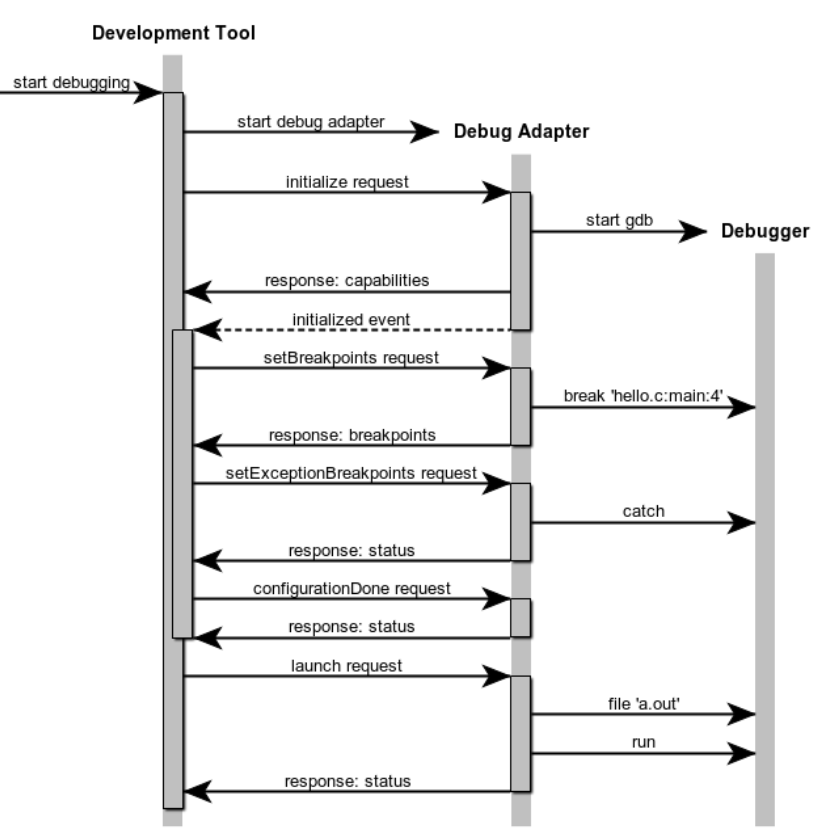
\includegraphics[width=0.7\columnwidth]{images/init-launch.png}
    \caption{Esempio di avvio di una sessione di debug\cite{DAP}}
\end{figure}

Quando inizia una sessione di debug, lo strumento di sviluppo deve comunicare con l'adattatore di debug che implementa il Protocollo di Adattatore di Debug (Debug Adapter Protocol, DAP). Il protocollo di base é implementato tramite lo scambio di messaggi composti da un'intestazione e un contenuto, chiamati \codeword{ProtocolMessage}. 
\begin{figure}[H]
    \lstinputlisting[language=JavaScript]{code/protocolMessage.txt}
    \caption{ProtocolMessage\cite{DAPmessage}}
\end{figure}

\subsubsection*{Termine della sessione di debug}

Il processo per terminare la sessione è diverso a seconda di come si é avviata la sessione, "avviato" o "agganciata":

\begin{itemize}
    \item {
        debugger "avviato": se il Debug Adapter implementa la richiesta di interruzione, allora la sessione viene terminata correttamente. Se non dovesse essere supportata la sessione continua a essere attiva fino a quando il debugger stesso non invia il comando di terminazione forzata
    }
    \item {
        debugger "agganciato": l'applicazione di debug  invia una richiesta di disconnessione al Debug Adapter. Questo permette al debugger di cessare la connessione con l'applicativo e continuare l'esecuzione
    }
\end{itemize}

se la sessione di debug termina, e il Debug Adapter è opportunamente configurato, un messaggio di corretta terminazione di sessione viene inviato all'applicazione di debug del programmatore.

\begin{figure}[H]    
    \centering
    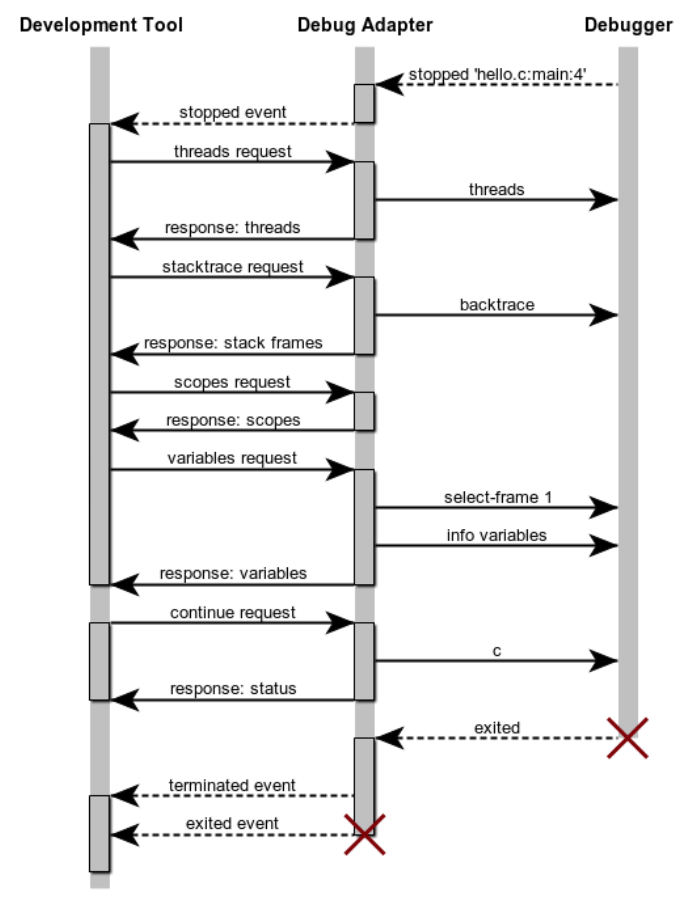
\includegraphics[width=0.7\columnwidth]{images/stop-continue-terminate.png}
    \caption{Esempio terminazione di una sessione di debug\cite{DAP}}
\end{figure}

\subsection{Logpoints}
I logpoint sono una variante dei breakpoint. Permettono, senza interrompere l'esecuzione, di controllare il valore di una o più variabili e mostrando il risultato nell console di debug di VSCode. Sono molto utili per evitare aggiungere codice di log all'interno del programma.

\section{Webview di VS Code}

VSCode mette a disposizione la possibilitá di creare nuove schede nelle quali un utente può visializzare contenuti personalizzati. Le webview sono molto simili a \codeword{iframe} e sono capaci di renderizzare ualsiasi contenuto HTML e scambio di informazioni tra la webview e VSCode. 

\begin{figure}[H]
    \centering
    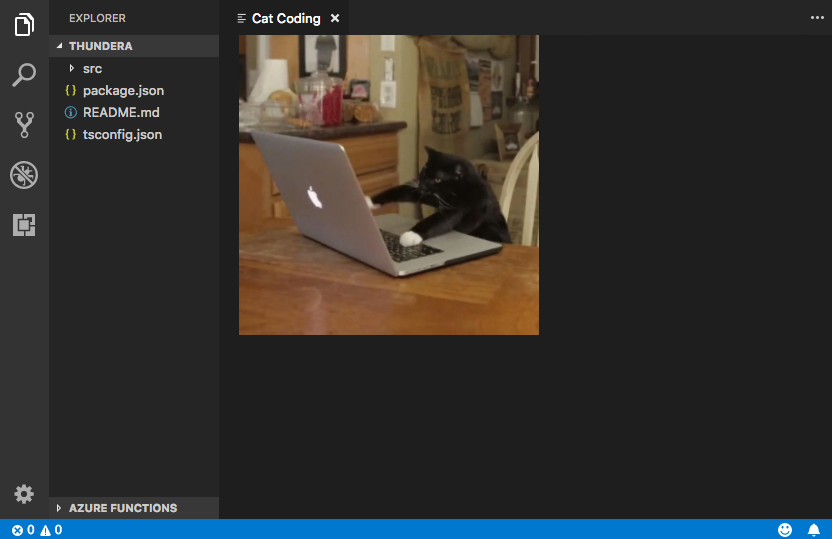
\includegraphics[width=0.7\columnwidth]{images/cat_coding.png}
    \caption{Esempio di una webview in VSCode}
    \label{fig:webcat}
\end{figure}

\chapter{Implementazione}
Per realizzare la nostra estensione andremo a estendere le funzionalità di base del debugger di VSCode. I comandi di base verranno gestiti dal debugger di VSCode dopo aver configurato opportunamente il collegamento con il GDB. La nostra estensione 
si occuperà di inviare comandi per la visualizzazione dei processi attualmente in esecuzione e mostrare i dati in una webview di VSCode.

\begin{figure}[H]
    \centering
    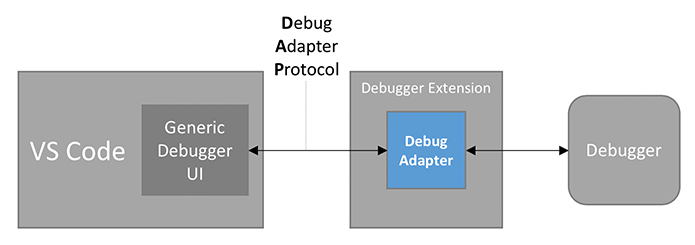
\includegraphics[width=0.7\columnwidth]{images/debug-arch2.png}
    \caption{Estensione del DP}
    \label{fig:dap dp and extension}
\end{figure}

Prima di instaurare un collegamento con il GDB vi è la necessità di compilare ed eseguire il nucleo nella macchina QEMU. VSCode mette a disposizione il file \codeword{./vscode/task.json} all'interno della cartella di lavoro. Il file permette di dichiarare dei comandi che permettono di automatizzare una moltitudine di operazioni.
\subsection*{task.json}
Il file \codeword{task.json} è in formato \codeword{JSON}. I campi che lo compongono sono spiegati esaustivamente all'interno della pagina dedicata della documentazione di VSCode \cite{VSCodeTasks}. In particolare si è configurato il file per eseguire i comandi di \codeword{compile} e \codeword{boot} presenti nell'ambiente di sviluppo Linux.  

\subsubsection*{compilazione}   

\begin{figure}[H]
    \lstinputlisting[language=sh]{code/task_compile.txt}
    \caption{Compilazione}
\end{figure}

\begin{itemize}
    \item \codeword{label}: identifica univocamente il nome del task all'interno dell'ambiente
    \item \codeword{type}: come deve essere interpretato il campo \codeword{command}, in questo caso come un comando di shell
    \item \codeword{command}: il comando effettivo da eseguire
    \item \codeword{group}: definisce il gruppo a cui il task appartiene all'interno di VSCode
    \item \codeword{presentation}: sono istruzioni per VSCode su come mostrare l'output del comando all'utente 
\end{itemize}

\subsubsection*{Avvio in modalità debug}   

\begin{figure}[H]
    \lstinputlisting[language=sh]{code/task_debug.txt}
    \caption{Avvio in modalità debug}
\end{figure}

Il task di avvio in modalità debug di QEMU del nucleo richiede un campo aggiuntivo per segnalare a VSCode la terminazione del task. QEMU viene avviato in modalità debug e resta in attesa fino alla connessione del GDB. Il campo \codeword{problemMatcher} è configurato in modo tale da attendere che QEMU segnali l'attesa del GDB tramite la riga di output \codeword{INF Attendo collegamento da gdb} .

\section{Build e connessione al nucleo}
Il prerequisito per il funzionamento dell'estensione è il collegamento al GDB. Per configurarlo è stato creato il file di configurazione \codeword{launch.json} all'interno della cartella \codeword{./.vscode} dell'ambiente di lavoro. 

\subsection*{lauch.json}

\begin{figure}[H]
    \lstinputlisting[language=sh]{code/launch_conf.txt}
    \caption{launch.json}
\end{figure}

\begin{itemize}
    \item \codeword{name}: identifica univocamente il nome della configurazione del debugger
    \item \codeword{type}: richiede la tipologia di debugger da utilizzare
    \item \codeword{request}: richiede di lanciare una nuova istanza del debugger
    \item \codeword{program}: indica quale eseguibile deve lanciare il debugger
    \item \codeword{cwd}: imposta il percorso di lavoro del debugger
    \item \codeword{miDebuggerPath}: è l'eseguibile del debugger da avviare
    \item \codeword{preLaunchTask}: richiede quali task eseguire prima di lanciare la connessione
    \item \codeword{setupCommands}: è la lista dei comandi da eseguire all'avvio del debugger
\end{itemize}

\subsubsection*{.gdbinitvscode}
GDB permette inoltre di caricare dei file di configurazione al cui interno sono definiti dei comandi di GDB, viene utilizzato per impostare le varie funzioni di visualizzazione, caricamento di ulteriori simboli o caricamento degli script personali. 

\begin{figure}[H]
    \lstinputlisting[language=sh]{code/gdbinit.txt}
    \caption{.gdbinitvscode}
\end{figure}

\section{nucleo\textunderscore vscode.py}

Il file \codeword{nucleo_debug.py} contiene la definizione di un nuovo comando per GDB: \codeword{process list}. Il comando è stato creato modificando la struttura dello script \codeword{nucleo.py}. 

\begin{figure}[H]
    \lstinputlisting[language=python]{code/nucleo.txt}
    \caption{nucleo.py}
\end{figure}

Il codice è stato modificato in modo tale da costruire come output un oggetto \codeword{JSON}

\begin{figure}[H]
    \lstinputlisting[language=python]{code/nucleo_vscode.txt}
    \caption{nucleo\textunderscore vscode.py}
\end{figure}

Il comando \codeword{process list} restituisce la lista di tutti i processi in esecuzione e le informazioni relative al contesto del processo.

\section{Estensione Nucleo Debug}
Il funzionamento generale dell'estensione si basa sull'ascoltare quando VSCode avvia una sessione di debug. Una volta avviato il debug viene caricata una webview, questa viene aggiornata a intervalli regolari lanciando i comandi personalizzati di GDB e formattando in HTML il risultato ottenuto dal debugger. 

\subsection{Creazione dell'estensione}
Dopo aver inizializzato l'ambiente di sviluppo per un estensione di VSCode grazie a \codeword{yeoman}, si procede alla configurazione del file di descrizione dell'estensione \codeword{package.json}. All'interno si possono definire vari campi tra cui:

\begin{itemize}
    \item \codeword{name}: identifica univocamente il nome dell'estensione
    \item \codeword{commands}: vettore di eventuali comandi che fornisce l'estensione 
    \item \codeword{activationEvents}: vettore di eventi da monitorare ai quali l'estensione viene caricata
\end{itemize}

in particolare \codeword{activationEvents} è stato popolato con l'evento \linebreak \codeword{onDebugResolve:cppdbg}, che permette di caricare l'estensione solo quando viene attivato il debug con tipo \codeword{cppdbg}.

\subsection{Caricamento dell'estensione}
VSCode, durante caricamento dell'estensione cerca nel file principale, \linebreak \codeword{extension.ts}, la funzione \codeword{activate()} e la chiama. All'intero della funzione è possibile trovare il codice di inizializzazione per le funzionalitá aggiuntive di debug.

\begin{figure}[H]
    \lstinputlisting[language=JavaScript]{code/activation.txt}
    \caption{activate()}
\end{figure}


\begin{itemize}
    \item \codeword{vscode.debug.onDidStartDebugSession}: permette di monitorare quando viene avviata una sessione di debug e chiamare una funzione che inizializza la webview contenente le informazioni del nucleo
    \item \codeword{vscode.debug.onDidTerminateDebugSession}: permette di monitorare quando viene terminata la sessione di debug e chiamare la funzione per pulire le schede aperte dall'estensione
\end{itemize}

\subsection{Richiesta del comando GDB}
All'interno del costruttore di \codeword{NucleoInfo} impostiamo un intervallo tramite \linebreak \codeword{setInterval(...)}, che si occuperà di gestire tutte le richieste dei comandi personalizzati di GDB tramite \codeword{customCommand(...)} e aggiornare la webview. 

\begin{figure}[H]
    \lstinputlisting[language=JavaScript]{code/costruttore.txt}
    \caption{NucleoInfo.constructor}
\end{figure}

\subsubsection{customCommand()}
\begin{figure}[H]
    \lstinputlisting[language=JavaScript]{code/customcommand.txt}
    \caption{NucleoInfo.customCommand()}
\end{figure}

La funzione \codeword{customCommand(...)} preleva il frame di esecuzione del Nucleo da GDB e dopo aver costruito il comando da eseguire crea una richiesta al Debug Adapter tramite il metodo \codeword{.customRequest}, il quale istanza una classe \codeword{ProtocolMessage} definita dal Debug Adapter Protocol di tipo \codeword{request} per richiedere l'esecuzione del commando da parte del GDB. 

\subsection{Webview}
Dopo aver recuperato tutte le informazioni del Nucleo necessarie viene chiamato il metodo \codeword{_getHTMLForWebview()}. 

\begin{figure}[H]
    \lstinputlisting[language=JavaScript]{code/htmlconstruct.txt}
    \caption{NucleoInfo.\textunderscore getHTMLforwebview}
\end{figure}

Per costruire la pagina HTML che verrà caricata dalla webview utilizziamo la libreria di templating \codeword{handlebars}. Tale libreria permette di sbrogliare il JSON ricevuto e creare dinamicamente il codice HTML per la visualizzazione dei dati. 

Il codice HTML generato viene assegnato alla webview che si preoccupa di disegnare la pagina ottenendo il risultato mostrato in figura
 
\begin{figure}[H]    
    \centering
    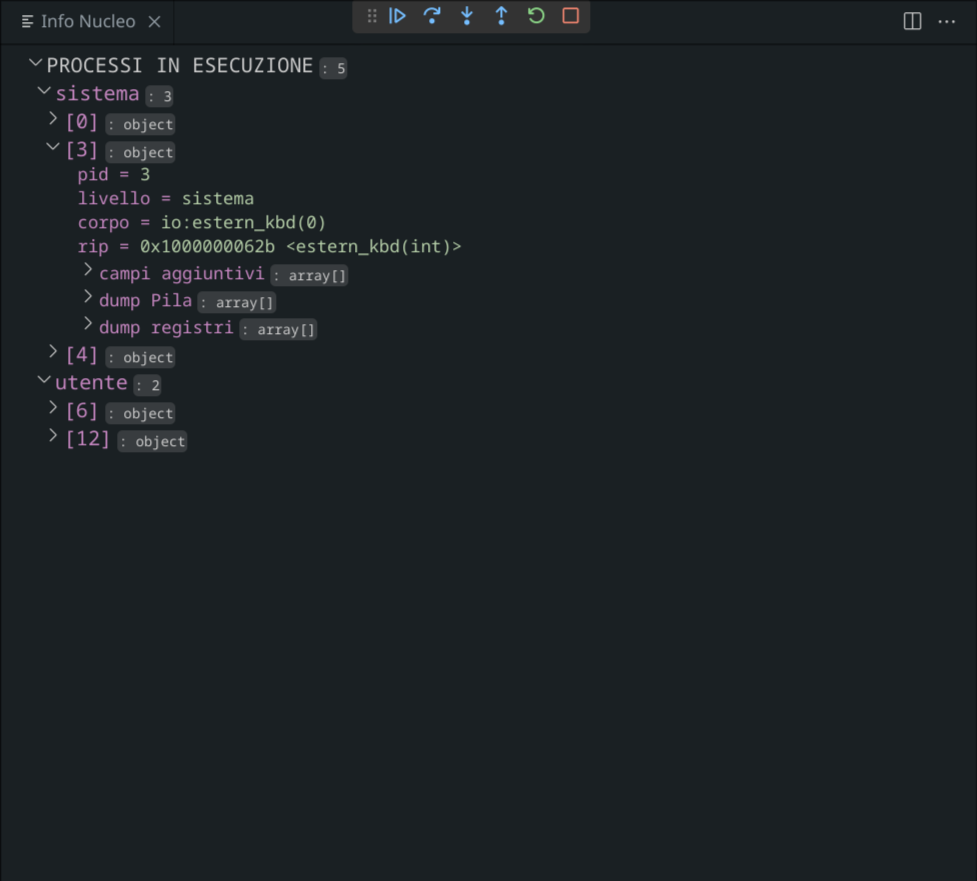
\includegraphics[width=0.7\columnwidth]{images/processes.png}
    \caption{Lista dei processi in esecuzione}
\end{figure}
\chapter{Utilizzo del debugger}
È possibile avviare l'interfaccia di debug tramite l'apposita scheda \ref{fig:startDebug} (pin 1) e poi dopo aver selezionato la configurazione \codeword{launch nmd}  dal menù a tendina \ref{fig:startDebug} (pin 2)si avvia la sessione premendo il tasto di avvio collocato accanto allo stesso menù.  

\begin{figure}[H]
    \centering
    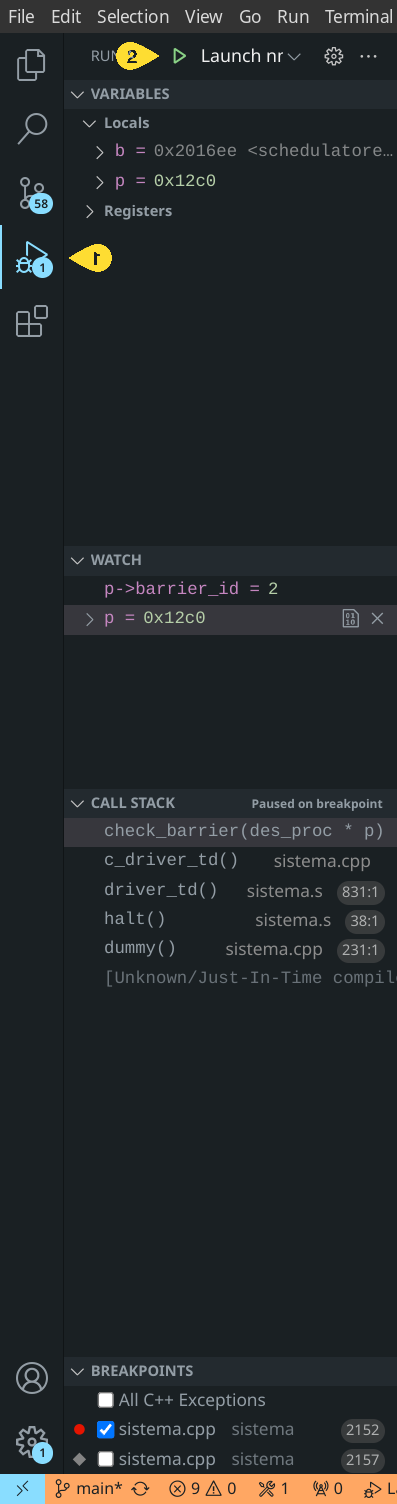
\includegraphics[height=0.3\pdfpageheight]{images/startDebug.png}
    \caption{Azioni per avviare il debug}
    \label{fig:startDebug}
\end{figure}

oppure premendo il tasto \codeword{F5} sulla tastiera.

L'interfaccia che ci viene presentata è la seguente 

\begin{figure}[H]
    \centering
    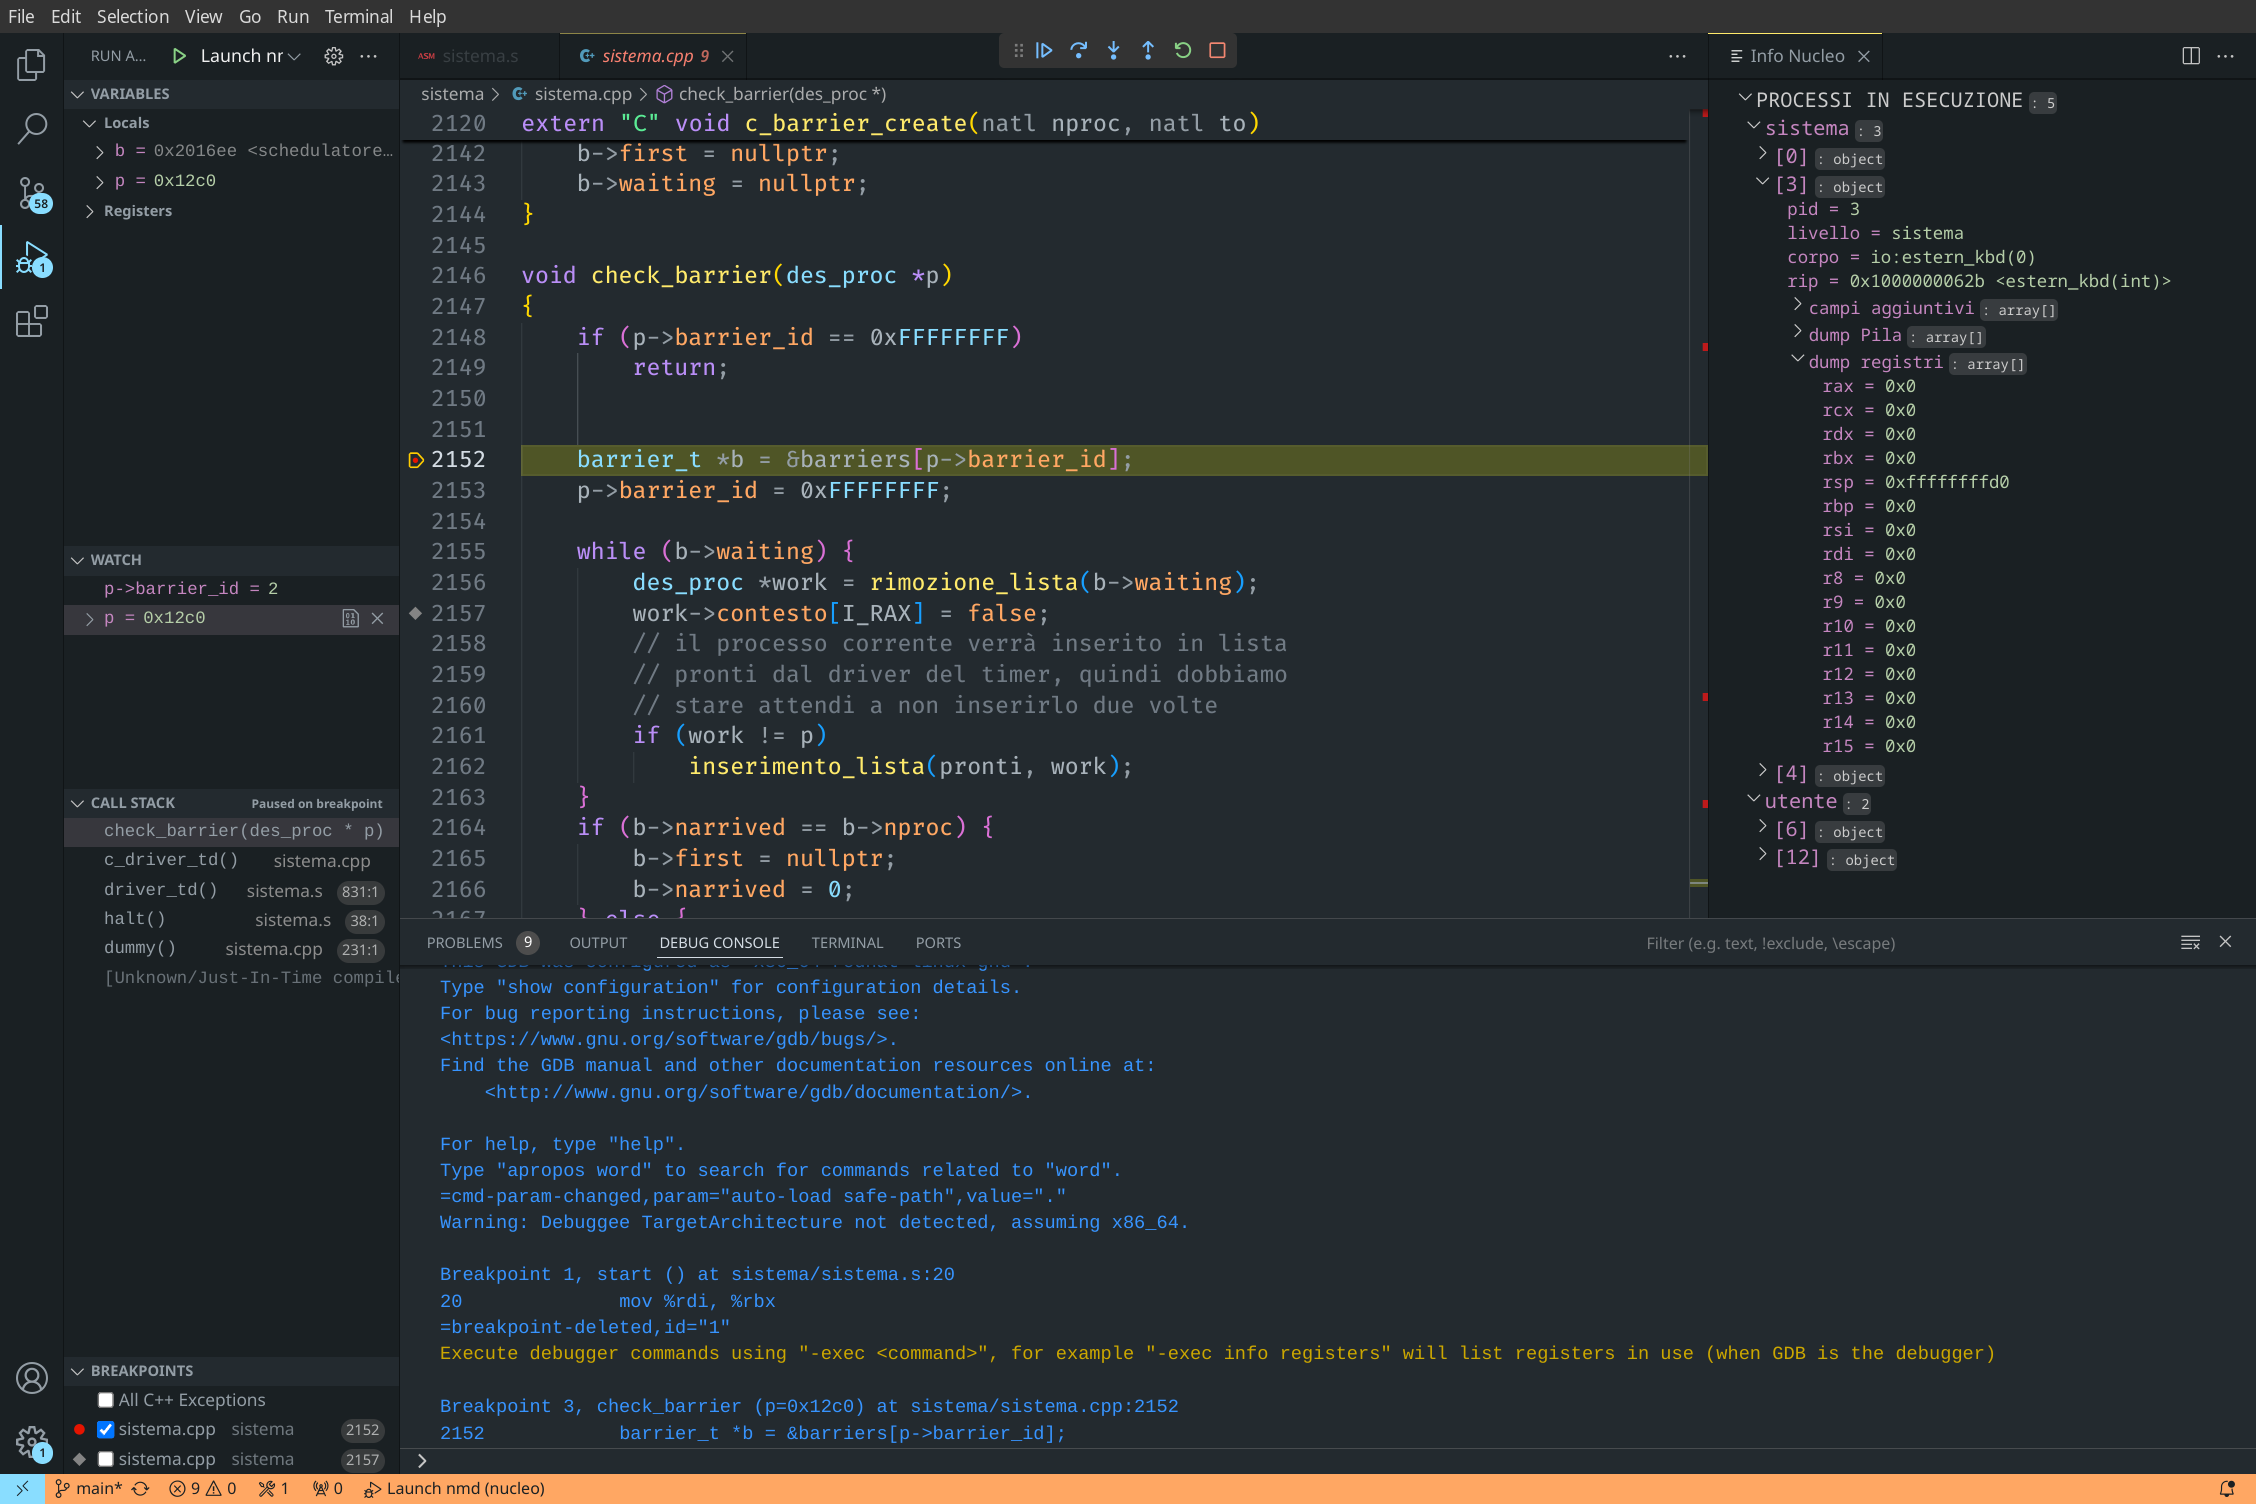
\includegraphics[width=\columnwidth]{images/fullDebug.png}
    \caption{Interfaccia di debug di  VSCode}
    \label{fig:debug screen}
\end{figure}

Analizziamo le varie finestre che ci vengono proposte.

\section{Breakpoint e Logpoint}
Nella vista del codice sorgente è possibile inserire un breakpoint premendo sul lato sinistro del numeri di rigainteressato, VSCode stesso si occuperà poi di comunicare al Debug Adapter la richiesta di inserimento del breakpoint.

\begin{figure}[H]
    \centering
    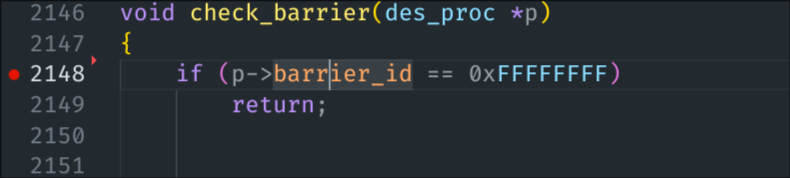
\includegraphics[width=0.7\columnwidth]{images/breakpoint_vscode.png}
    \caption{Esempio di un breakpoint in VSCode}
    \label{fig:breakpoint}
\end{figure}

Similarmente si può inserire un logpoint premendo con il tasto destro del mouse e selezionando la dicitura logpoint. All'interno del box di testo si possono aggiungere le variabili da osservare tramite \codeword{{{variable}}}

\begin{figure}[H]
    \centering
    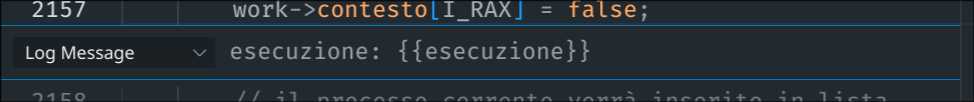
\includegraphics[width=0.7\columnwidth]{images/logpoint.png}
    \caption{Esempio di logpoint}
    \label{fig:logpoint}
\end{figure}

una volta ripresa l'esecuzione del codice possiamo vedere l'output nella console di debug.

\section{Azioni di debug}

VSCode mette a disposizione una barra di funzioni \ref*{fig:middleDebug}(pin 1) per permettere all'utente di ispezionare il codice tramite i comandi di step over, step in e step out. È possibile anche eseguire azioni come continue, stop e il riavvio della sessione di debug.  

\begin{figure}[H]
    \centering
    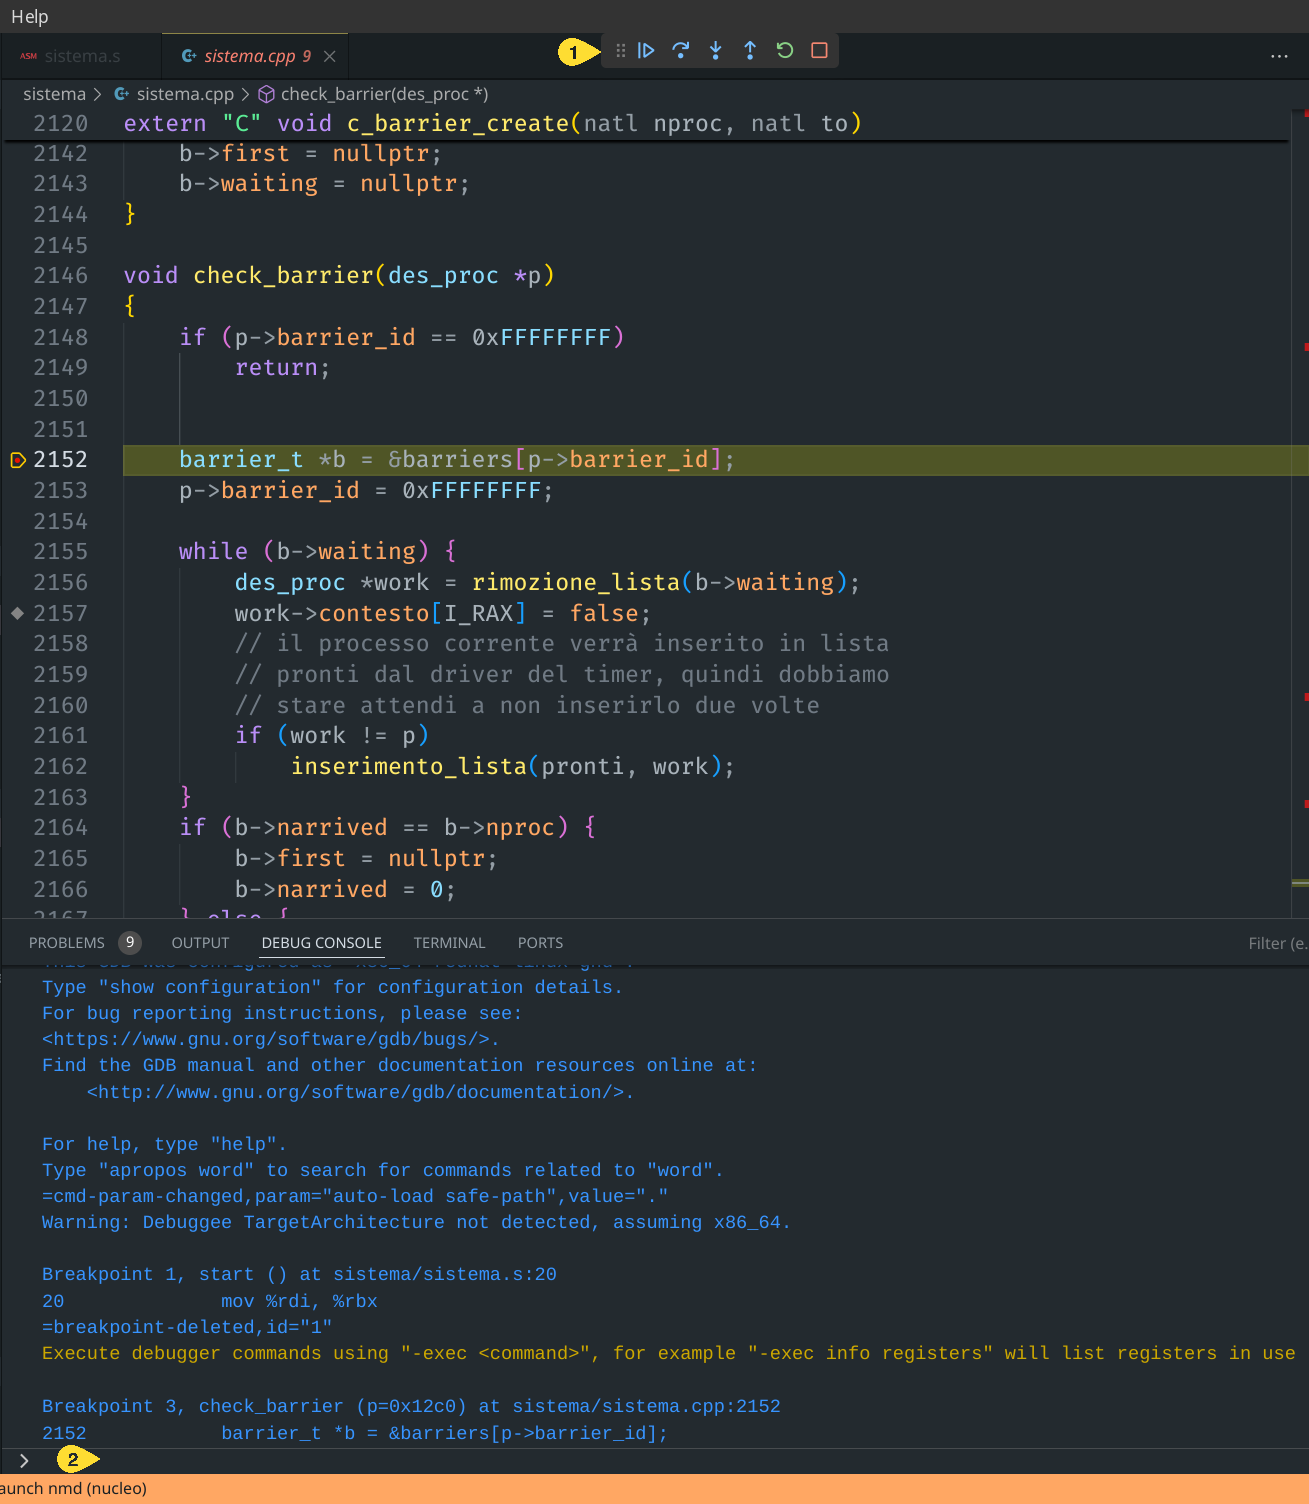
\includegraphics[width=0.8\columnwidth]{images/middle_debug.png}
    \caption{Azioni e linea di comando}
    \label{fig:middleDebug}
\end{figure}

Inoltre è possibile inviare comandi di GDB direttamente dalla linea di comando \ref*{fig:middleDebug}(pin 2) tramite il comando \codeword{-exec [GDB command]}.

\section{Pannello di sinistra}

Il pannello di sinistra permette di analizzare lo stato delle variabili locali \ref*{fig:leftDebug}(pin 2) e lo stato dei registri \ref*{fig:leftDebug}(pin 3).

\begin{figure}[H]
    \centering
    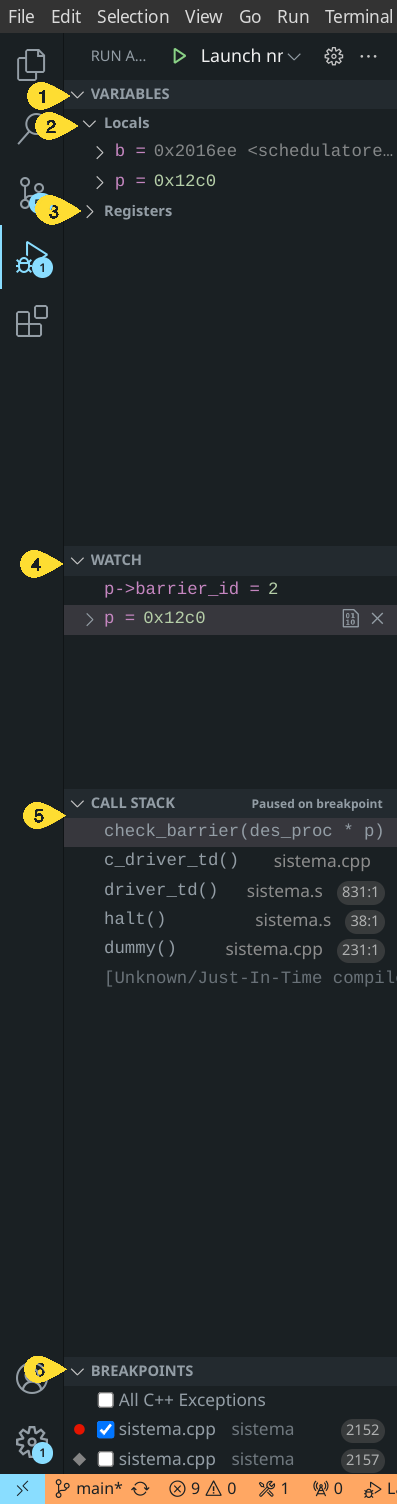
\includegraphics[height=0.4\pdfpageheight]{images/leftDebug.png}
    \caption{Azioni e linea di comando}
    \label{fig:leftDebug}
\end{figure}

\subsection*{Watch}
Nel pannello dedicato \ref*{fig:leftDebug}(pin 4) possiamo visualizzare le variabili messe sotto osservazione. L'aggiunta può avvenire tramite il pulsante "+" oppure selezionando con il cursore la variabile o l'espressione da analizzare e cliccando con il tasto destro dal menù a tendina selezionare "Add to watch" come mostrato in figura.

\begin{figure}[H]
    \centering
    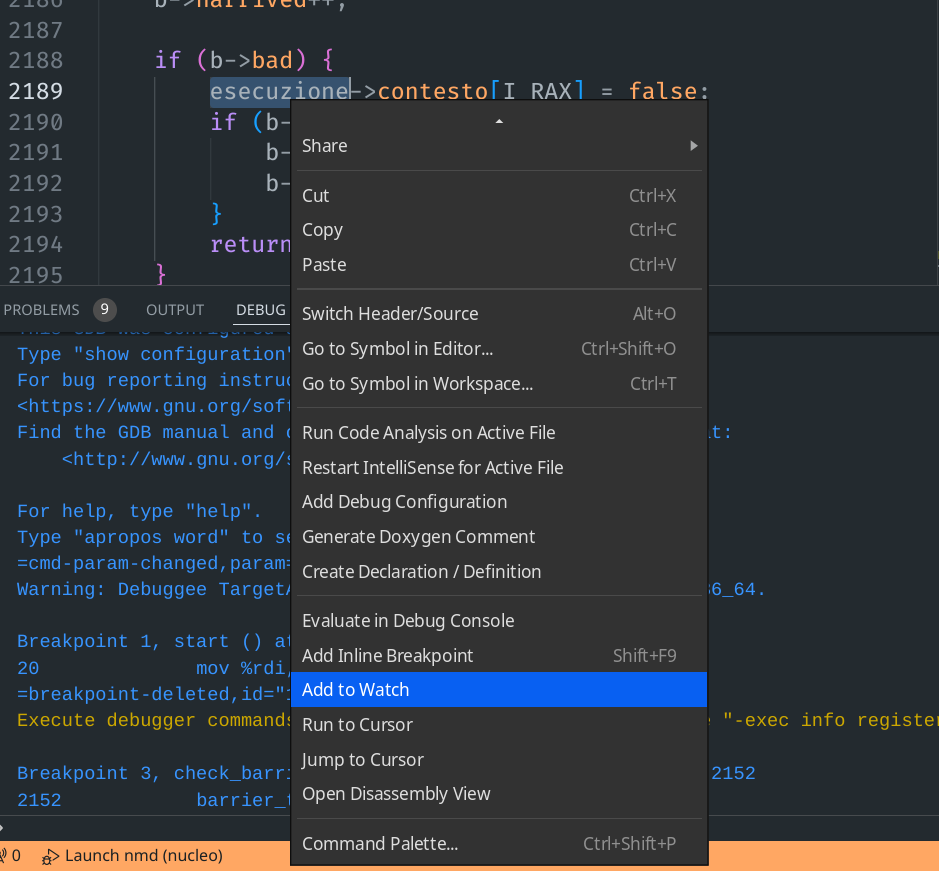
\includegraphics[width=0.8\columnwidth]{images/addWatch.png}
    \caption{Aggiunta al watch di una variabile}
    \label{fig:watchvariabili}
\end{figure}

\subsection*{Call stack e breakpoints}
È inoltre possibile visualizzare informazioni riguardanti il call stack \ref*{fig:leftDebug}(pin 5) e gestire i breakpoint presenti tramite il pannello dedicato \ref*{fig:leftDebug}(pin 6)

\section{Informazioni aggiuntive}

Sulla parte destra della finestra di debug troviamo la scheda dedicata alle informazioni aggiuntive del Nucleo. In questo caso
mostra solo i processi in esecuzione 

\begin{figure}[H]
    \centering
    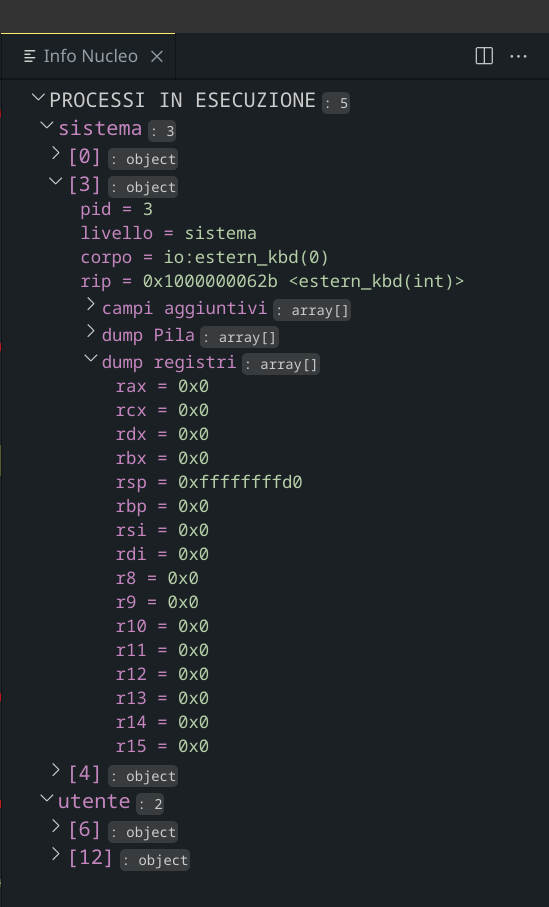
\includegraphics[height=0.3\pdfpageheight]{images/infoNucleo.png}
    \caption{Informazioni aggiuntive sul nucleo}
    \label{fig:infoNucleo}
\end{figure}

\subsection*{Processi in esecuzione}
Le informazioni relative ai processi vengono mostrate tramite una lista con elementi selezionabili. Ogni elemento della lista è formato da una rappresentazione tramite \codeword{chiave:valore} e un eventuale campo adiacente con eventuali informazioni sulla tipologia della variabile o oggetto. I processi sono stati divisi per convenienza tra processi di sistema e processi utente. 




\chapter{Conclusione e sviluppi futuri}
L'utilizzo dell'estensione facilita l'approccio al debug e in particolare al Nucleo didattico. Tuttavia l'estensione non è completa, vi sono numerose funzionalità che possono essere implementate per ampliare le informazioni relative al Nucleo, come ad esempio informazioni riguardanti la memoria virtuale o stato dell'APIC.

\chapter{Sviluppo e contributi}
In questo capitolo viene spiegato come è possibile aggiungere nuove funzionalità all'estensione. È possibile sviluppare l'estensione tramite la macchina virtuale fornita durante il corso di Calcolatori Elettronici, tuttavia è consigliato vivamente di installare il Nucleo sulla propria macchina seguendo le istruzioni fornite dal Professor Lettieri\cite{mainsite}. Come editor è molto consigliato VSCode stesso in quanto è configurato per debug e esecuzione delle estensioni.

\section*{Installazione}
Per prima cosa bisogna impostare l'ambiente di sviluppo per l'estensione:
\begin{itemize}
    \item scaricare la repository del progetto \href{google.com}{Nucleo-Debugger} 
    \item navigare all'interno della repository
    \item creare la propria branch di sviluppo della feature da implementare tramite \codeword{git}
    \item installare le dipendenze: \codeword{yarn} e \codeword{node}
    \item inizializzare l'ambiente con il comando \codeword{yarn install} e una volta terminato lanciare il comando \codeword{yarn global add vsce} per installare il pacchetto di VSCode per creare il file di installazione dell'estensione
    \item aprire VSCode con il comando \codeword{code .}
\end{itemize}

Se eventualmente l'estensione per il debug del nucleo dovesse essere presente tra le estensioni di VSCode bisogna rimuoverla.

\subsection*{Debug e esecuzione}
È possibile caricare l'estensione in un ambiente separato da quello di sviluppo tramite proprio il debugger di VSCode premendo il tasto \codeword{F5}. Una volta completata la compilazione verrà avviata una nuova finestra di VSCode dove apriamo la cartella del Nucleo, in questo caso possiamo usare \codeword{prova-test} e avviare a sua volta il debug tramite \codeword{F5}.

\section{Aggiunta di comandi}
Per aggiungere comandi bisogna modificare il file \codeword{NucleoInfo.ts} nelle sezioni indicate:
\begin{itemize}
    \item {
        se vi è la necessità di ricevere dati da GDB bisogna dichiarare una variabile di supporto.
        \begin{figure}[H]
            \lstinputlisting[language=JavaScript]{code/var.txt}
            \caption{Variabile di supporto per i dati}
        \end{figure}
    }
    \item {
        Per eseguire un comando è necessario chiamare la funzione \linebreak \codeword{.customCommand(args ...)} e se si devono ricevere dati dal GDB si può assegnare il valore di ritorno della funzione alla relativa variabile di appoggio.
        \begin{figure}[H]
            \lstinputlisting[language=JavaScript]{code/command_exec.txt}
            \caption{Richiesta di esecuzione del comando}
        \end{figure}
    }
    \item {
        Per aggiornare la webview bisogna aggiungere all'HTML già presente il proprio tramite  una funzione di appoggio che si occupa di formattare i dati (es. \codeword{this.YOUR_FORMATTER()})
        \begin{figure}[H]
            \lstinputlisting[language=JavaScript]{code/getHTML.txt}
            \caption{Costruzione della pagina HTML}
        \end{figure}
    }
    \item {
        il formattatore deve creare il codice HTML da incorporare nella funzione \codeword{_getHtmlForWebview()} per mostrare correttamente i dati
        \begin{figure}[H]
            \lstinputlisting[language=JavaScript]{code/formatter.txt}
            \caption{Implementazione di un formattatore}
        \end{figure}
        Le strutture per lo scambio di informazioni sono a discrezione del programmatore, tuttavia si consiglia l'utilizzo del formato \codeword{JSON} per facilitare la visualizzazione tramite il tool di templating handlebars\cite{handlebars}.
    }
\end{itemize}
\subsection{nucleo\textunderscore vscode.py}
All'interno del file \codeword{nucleo_vscode.py} bisogna implementare il nuovo comando richiesto dall'estensione. Per l'effettiva implementazione del comando dipende dalla funzione che si vuole aggiungere, si faccia riferimento alla guida per lo scripting di GDB\cite{GDBpython} e al file \codeword{./debug/nucleo.py} all'interno di una delle versioni del nucleo presenti sul sito del Professor Lettieri \cite{testiEsame}.  

% \href[options]{https://github.com/microsoft/vscode-cpptools/blob/main/Documentation/Building%20the%20Extension.md}{Build istructions microsoft}

%\href[options]{https://stackoverflow.com/questions/56237448/how-to-make-acquirevscodeapi-available-in-vscode-webview-react}{se si vuole le API di vscode nel javascript}
%\href[options]{https://www.codemag.com/Article/1809051/Writing-Your-Own-Debugger-and-Language-Extensions-with-Visual-Studio-Code}{Come scrivere il proprio language support e debug}
%\href[options]{https://stackoverflow.com/questions/59040679/how-to-output-stopped-events-in-visual-studio-code-debugger#59068740}{implementare lo stopped event}
%
%\href[options]{https://stackoverflow.com/questions/56012353/how-to-get-vs-code-debug-data-like-breakpoints-steps-line-code/63657824#63657824}{Debug tracker}
%\href[options]{https://github.com/Microsoft/vscode/issues/62843}{Debug tracker API}
%
%\href[options]{https://stackoverflow.com/questions/59040679/how-to-output-stopped-events-in-visual-studio-code-debugger}{stopOnStep listener}



% Rimuovere se non si vuole la tabella delle figure
% \listoffigures

\chapter{Ringraziamenti}


\appendix
\bibliography{chapters/bibliografia.bib}
\bibliographystyle{plainnat}

\end{document}
% -----------------------------------------------------------------
